\begin{esercizio}
   An electron is under the action of a constant magnetic field $\vb{B}=B_z(0,0,1)$. At $t=0$ a magnetic field along the $\hat{x}$ direction is turned on; its strength increases uniformly from $0$ to $B_x$ at time $t=T$ and then remains constant. The electron is initially in the spin-up state. Assume $B_x \ll B_z$.
   \begin{enumerate}[label=\alph*), leftmargin=0.6cm]
      \item Find the transition amplitude to the spin-down state at $t=T$ in the first order of perturbation theory.
      \item Calculate with a good approximation the transition probability for $B_z=5 \cdot 10^6 \rm \; V/m$, $B_x=10^5 \rm \; V/m$ and $T=\frac{mc}{e B_x}$. Is perturbation theory valid?
      \item Calculate in eV the first nonzero correction to the energy levels for $t \gg T$.
   \end{enumerate}
\end{esercizio}
\begin{soluzione}
   Sappiamo che, in generale, l'hamiltoniana di una particella in un campo magnetico è
   \begin{equation*}
      H=-\vb*{\mu} \vdot \vb{B}
   \end{equation*}
   dove $\vb*{\mu}$ è il momento magnetico della particella. Nel caso di un elettrone, il momento magnetico è dato da
   \begin{equation*}
      \vb*{\mu}
      =\frac{\hbar e}{2 m c} \vb*{\sigma}
   \end{equation*}
   dove $\vb*{\sigma}$ sono le matrici di Pauli.\\
   Analizziamo adesso il problema. Inizialmente abbiamo l'azione di un campo magnetico costante diretto lungo $\hat{z}$, dunque l'hamiltoniana assume la forma
   \begin{equation*}
      H_0=-\frac{\hbar e}{2 m c} B_z \sigma_z
   \end{equation*}
   Ricordiamo che la matrice di Pauli $\sigma_z$ è definita come
   \begin{equation*}
      \sigma_z
      =
      \begin{pmatrix}
         1 & 0 \\
         0 & -1
      \end{pmatrix}
   \end{equation*}
   e dunque i livelli energetici sono
   \begin{equation*}
      E_{\uparrow}=\frac{\hbar e B_z}{2 m c}
      \qq{e}
      E_{\downarrow}=-\frac{\hbar e B_z}{2 m c}
   \end{equation*}
   Osserviamo che il ground state è quello con spin down, dunque $E_0=E_{\downarrow}$, mentre il primo stato eccitato è quello con spin up, dunque $E_1=E_{\uparrow}$. Inoltre tra i due stati c'è uno splitting in energia pari a $\Delta E=\frac{\hbar e B_z}{mc}$.\\
   Questa è la situazione prima del tempo $t=0$; una volta raggiunto tale istante viene accesso un campo magnetico che varia linearmente, dunque nella forma $B(t)=mt + q$. In particolare, sappiamo che $B_x(0)=0 \equiv q$ e $B_x(T)=B_x$, per cui il coefficiente angolare è dato da $m=B_x/T$. In definitiva l'espressione generale di tale campo è
   \begin{equation*}
      B(t)=\frac{B_x}{T}t
   \end{equation*}
   Possiamo adesso svolgere il punto a). Poiché tale campo dipende dal tempo, ci troviamo nel caso di teoria perturbativa dipendente dal tempo e dobbiamo calcolare l'ampiezza di transizione dovuta a questo campo magnetico. L'ampiezza di transizione dallo stato iniziale $\ket*{i}=\ket*{\uparrow}$ allo stato finale $\ket*{f}=\ket*{\downarrow}$ sarà
   \begin{equation}
      c_{i \to f}(T)
      =-\frac{i}{\hbar} \int_{0}^{T} \dd{t} e^{i \omega_{f,i} t} \, V_{f,i}
      \label{eq:ampiezza_di_transizione_al_tempo_T}
   \end{equation}
   dove
   \begin{equation}
      \omega_{f,i}
      =\frac{E_{\downarrow} - E_{\uparrow}}{\hbar}
      =-\frac{e B_z}{m c}
      \label{eq:omega_f_i_campo_magnetico}
   \end{equation}
   e $V_{f,i}=\mel*{\downarrow}{V(t)}{\uparrow}$. Calcoliamo tale elemento di matrice: dato che il potenziale che dobbiamo considerare è quello associato al campo magnetico lungo $x$, si ha
   \begin{equation*}
      V_{f,i}
      =\mel*{\downarrow}{\frac{\hbar e}{2 m c} \sigma_x B_x \frac{t}{T}}{\uparrow}
      =\frac{\hbar e}{2 m c} B_x \frac{t}{T}\mel*{\downarrow}{\sigma_x}{\uparrow}
   \end{equation*}
   Ricordiamo che $\sigma_x$ è definita come
   \begin{equation*}
      \sigma_x=
      \begin{pmatrix}
         0 & 1 \\
         1 & 0
      \end{pmatrix}
   \end{equation*}
   pertanto la sua azione è quella di scambiare gli stati up e down tra loro, per cui si ha che $\sigma_x \ket*{\uparrow}=\ket*{\downarrow}$ e quindi
   \begin{equation}
      V_{f,i}
      =\frac{\hbar e}{2 m c} B_x \frac{t}{T}
      \label{eq:elemento_di_matrice_campo_magnetico_variabile}
   \end{equation}
   in quanto $\braket*{\downarrow}=1$.\\
   Sostituendo la \eqref{eq:omega_f_i_campo_magnetico} e la \eqref{eq:elemento_di_matrice_campo_magnetico_variabile} nella \eqref{eq:ampiezza_di_transizione_al_tempo_T} otteniamo
   \begin{equation*}
      c_{i \to f}(T)
      =-\frac{i}{\hbar} \int_{0}^{T} \dd{t} e^{-i \frac{e B_z}{m c} t } \frac{\hbar e}{2 m c} B_x \frac{t}{T}
      =-i \frac{e B_x}{2 m c T} \int_{0}^{T} \dd{t} e^{-i \frac{e B_z}{m c} t } t
   \end{equation*}
   Ricordiamo che in generale si ha
   \begin{equation*}
      \int_{0}^{T} \dd{t} e^{- a t} t
      =\left. -\frac{1}{a} e^{-a t} t \right|_{0}^{T} + \frac{1}{a} \int_{0}^{T} \dd{t} e^{-a t}
      =-\frac{1}{a} e^{-a T} T - \frac{1}{a^2} \qty( e^{-a T} - 1 )
   \end{equation*}
   Nel nostro caso $a=-i \frac{e B_z}{m c}$, per cui
   \begin{equation}
      \begin{split}
         c_{i \to f}(T)
         & =-i \frac{e B_x}{2 m c T} \qty[ -i \frac{m c}{e B_z} e^{-i \frac{e B_z}{m c} T} T
         - \qty(\frac{m c}{e B_z})^2 \qty( e^{-i \frac{e B_z}{m c} T} - 1 ) ]
         \\[0.1cm]
         & =\frac{1}{2} \frac{B_x}{B_z} e^{-i \frac{e B_z}{m c} T}
         - i \frac{m c}{2 e T} \frac{B_x}{B_z^2} \qty( e^{-i \frac{e B_z}{m c} T} - 1 )
      \end{split}
      \label{eq:ampiezza_di_transizione_up_to_down_al_tempo_T}
   \end{equation}
   Passiamo al quesito b). Dobbiamo calcolare, con una buona approssimazione, la probabilità in corrispondenza dei valori forniti dal testo. Osserviamo innanzitutto che, sfruttando l'espressione che ci viene fornita per $T$, la \eqref{eq:ampiezza_di_transizione_up_to_down_al_tempo_T} diventa
   \begin{equation}
      c_{i \to f}(T)
      =\frac{1}{2} \frac{B_x}{B_z} e^{-i \frac{B_z}{B_x}}
      - \frac{i}{2} \qty(\frac{B_x}{B_z})^2 \qty( e^{-i \frac{B_z}{B_x}} - 1 )
      \label{eq:ampiezza_di_transizione_up_to_down_al_tempo_T_dopo_sostituzione}
   \end{equation}
   Notiamo che nella \eqref{eq:ampiezza_di_transizione_up_to_down_al_tempo_T_dopo_sostituzione} il primo termine dipende linearmente dal rapporto $B_x/B_z$, mentre il secondo vi dipende quadraticamente. Poiché il testo ci dice di assumere che $B_x/B_z \ll 1$, possiamo trascurare il secondo termine e scrivere semplicemente
   \begin{equation*}
      c_{i \to f}(T)
      \approx \frac{1}{2} \frac{B_x}{B_z} e^{-i \frac{B_z}{B_x}}
   \end{equation*}
   Sostituendo adesso i valori forniti, la probabilità sarà data da
   \begin{equation*}
      P_{i \to f}
      =| c_{i \to f}(T) |^2
      =\frac{1}{4} \qty(\frac{B_x}{B_z})^2
      =\frac{1}{4} \qty(\frac{10^5}{5 \cdot 10^6})^2
      =\frac{1}{4} \qty(\frac{1}{50})^2
      =10^{-4}
   \end{equation*}
   Poiché abbiamo trovato che $P_{i \to f} \ll 1$, la teoria perturbativa è valida.\\
   Svolgiamo infine in quesito c). Dobbiamo calcolare la prima correzione non nulla sugli stati al tempo $t \gg T$. Notiamo che per tempi $t$ successivi all'istante $t=T$ il campo magnetico resta costante, dunque il problema può essere trattato come un problema di teoria perturbativa indipendente dal tempo.\\
   Il testo chiede in particolare correzione fino al primo ordine non nullo. Si trova infatti che al primo ordine della teoria perturbativa la correzione è nulla. Mostriamo esplicitamente ciò: ricordiamo innanzitutto che la correzione al primo ordine all'energia del generico livello $n$-esimo è data dall'elemento di matrice della perturbazione rispetto all'autostato $n$-esimo imperturbato:
   \begin{equation*}
      \delta E_n^{(1)}
      =\mel{\psi_n^{(0)}}{V}{\psi_n^{(0)}}
   \end{equation*}
   In particolare, per lo stato $\ket*{\downarrow}$ abbiamo che
   \begin{equation*}
      \delta E_{\downarrow}^{(1)}
      =\mel{\downarrow}{V}{\downarrow}
      \propto \mel{\downarrow}{\sigma_x}{\downarrow}
      =\braket{\downarrow}{\uparrow}
      =0
   \end{equation*}
   e con passaggi analoghi per lo stato $\ket*{\uparrow}$ si trova che
   \begin{equation*}
      \delta E_{\uparrow}^{(1)}
      =\mel{\uparrow}{V}{\uparrow}
      =0
   \end{equation*}
   Passiamo allora al secondo ordine, il quale è dato da
   \begin{equation*}
      \delta E_n^{(2)}
      =\mel{\psi_n^{(0)}}{V}{\psi_n^{(1)}}
   \end{equation*}
   dove $\ket*{\psi_n^{(1)}}$ è l'autostato corretto fino al primo ordine, il quale a sua volta è dato da
   \begin{equation*}
      \ket*{\psi_n^{(1)}}
      =\sum_{k \neq n} \frac{V_{k,n}}{E_n^{(0)} - E_k^{(0)}}
      \qq{dove}
      V_{k,n}=\mel*{\psi_n^{(0)}}{V}{\psi_k^{(0)}}
   \end{equation*}
   In questo caso abbiamo un sistema a due livelli, dunque la sommatoria si riduce ad un solo termine. Se ad esempio calcoliamo la correzione allo stato $\ket*{\uparrow}$, avremo che $n=\,\uparrow$ e $k=\,\downarrow$, dunque
   \begin{equation*}
      V_{\uparrow,\downarrow}
      =\mel{\uparrow}{V}{\downarrow}
      =\frac{\hbar e}{2 m c} B_x \mel{\uparrow}{\sigma_x}{\downarrow}
      =\frac{\hbar e}{2 m c} B_x
   \end{equation*}
   Per quanto riguarda la differenza di energie invece si ha:
   \begin{equation*}
      E_{\uparrow}^{(0)} - E_{\downarrow}^{(0)}
      =\frac{\hbar e}{m c} B_z
   \end{equation*}
   Per inciso, osserviamo che tale quantità è pari a\footnote{\E da notare che stiamo lavorando nel sistema CGS, ecco perché $B$ ha tali unità di misura. Inoltre il vantaggio di lavorare in tale sistema è che il prodotto $e B$ avrà lo stesso valore di $B$, misurato però in $\rm eV/m$.}
   \begin{equation*}
      E_{\uparrow}^{(0)} - E_{\downarrow}^{(0)}
      =\frac{\hbar c}{m c^2} e B_z
      =\rm \frac{200 \; eV \, nm \cdot 5 \cdot 10^6 \; eV}{5 \cdot 10^2 \; eV \cdot 10^9 \; nm}
      =2 \cdot 10^{-6} \; eV
   \end{equation*}
   Ne segue che la correzzione al primo ordine è
   \begin{equation*}
      \ket*{\psi_1^{(1)}}
      =\frac{\mel*{\uparrow}{V}{\downarrow}}{E_{\uparrow}^{(0)} - E_{\downarrow}^{(0)}} \ket*{\downarrow}
      =\frac{\frac{e \hbar}{2 m c} B_x}{\frac{e \hbar}{m c} B_z} \ket*{\downarrow}
      =\frac{1}{2} \frac{B_x}{B_z} \ket*{\downarrow}
   \end{equation*}
   dove lo abbiamo indicato con $\ket*{\psi_1^{(1)}}$ per enfatizzare il fatto che non si avrà più l'autostato $\ket*{\uparrow}$. Tale notazione non è ambigua perché quest'ultimo rappresenta il primo stato eccitato del sistema. Ne segue che l'autostato corretto fino al primo sarà dato da
   \begin{equation*}
      \ket*{\psi_1}
      =\ket*{\uparrow} + \ket*{\psi_1^{(1)}}
      =\ket*{\uparrow} + \frac{1}{2} \frac{B_x}{B_z} \ket*{\downarrow}
   \end{equation*}
   e in tale espressione si evince il mixing tra gli stati.\\
   Con passaggi analoghi, si trova che la correzione al primo ordine per il ground state è
   \begin{equation*}
      \ket*{\psi_0^{(1)}}
      =\frac{\mel*{\downarrow}{V}{\uparrow}}{E_{\downarrow}^{(0)} - E_{\uparrow}^{(0)}} \ket*{\uparrow}
      =\frac{\frac{e \hbar}{2 m c} B_x}{-\frac{e \hbar}{m c} B_z} \ket*{\uparrow}
      =-\frac{1}{2} \frac{B_x}{B_z} \ket*{\downarrow}
   \end{equation*}
   mentre lo stato corretto fino al primo ordine è
   \begin{equation*}
      \ket*{\psi_0}
      =\ket*{\downarrow} + \ket*{\psi_0^{(1)}}
      =\ket*{\downarrow} - \frac{1}{2} \frac{B_x}{B_z} \ket*{\uparrow}
   \end{equation*}
   Avendo trovato le correzioni agli stati al primo ordine, possiamo calcolare le correzione all'energia al secondo ordine. In particolare, per lo stato $\ket*{\uparrow}$ si ha
   \begin{equation*}
      \delta E_{\uparrow}^{(2)}
      =\mel*{\psi_1^{(0)}}{V}{\psi_1^{(1)}}
      =\frac{\hbar e}{2 m c} B_x \mel*{\psi_1^{(0)}}{\sigma_x}{\psi_1^{(1)}}
      =\frac{\hbar e}{4 m c} \frac{B_x^2}{B_z}
      %=\rm 2 \cdot 10^{-10} \; eV
   \end{equation*}
   mentre per lo stato $\ket*{\downarrow}$ si ha
   \begin{equation*}
      \delta E_{\uparrow}^{(2)}
      =\mel*{\psi_0^{(0)}}{V}{\psi_0^{(1)}}
      =\frac{\hbar e}{2 m c} B_x \mel*{\psi_0^{(0)}}{\sigma_x}{\psi_0^{(1)}}
      =-\frac{\hbar e}{4 m c} \frac{B_x^2}{B_z}
   \end{equation*}
   Calcoliamo tale quantità: si ha\footnote{Qualcosa non va, questo calcolo è sbagliato.}
   \begin{equation*}
      \frac{\hbar e}{4 m c} \frac{B_x^2}{B_z}
      =\frac{\hbar c}{4 m c^2} e B_x \frac{B_x}{B_z}
      =\rm \frac{200 \; eV \, nm}{4 \cdot 5 \cdot 10^2 \; eV} \cdot 10^5 \; eV \, nm^{-1} \cdot \frac{10^5 \; V \, nm^{-1}}{5 \cdot 10^6 \; V \, nm^{-1}}
      =2 \cdot 10^{-10} \; eV
   \end{equation*}
   Si vede come la correzione è piuttosto piccola rispetto al valore della differenza in energia tra i livelli, come del resto ci aspettavamo.\\
   Riassumiamo graficamente la situazione in termini di livelli energetici:
   \begin{figure}[H]
      \centering
      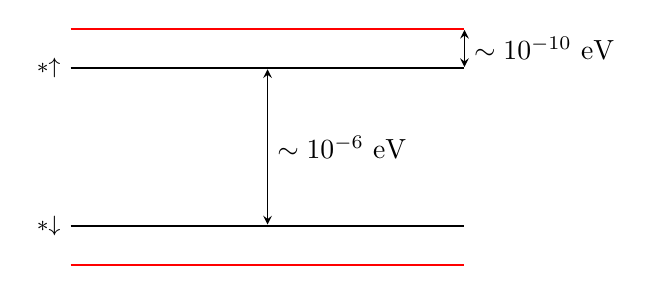
\begin{tikzpicture}
         \draw[thick] (-2.5,1) node[left] {\footnotesize $\ket*{\uparrow}$} -- (2.5,1);
         \draw[thick] (-2.5,-1) node[left] {\footnotesize $\ket*{\downarrow}$} -- (2.5,-1);
         \draw[stealth-stealth, shorten >= 0.4pt, shorten <= 0.4pt] (0,-1) -- (0,1) node[midway,right] {$\sim 10^{-6}$ eV};
         \draw[thick,red] (-2.5,1.5) -- (2.5,1.5);
         \draw[thick,red] (-2.5,-1.5) -- (2.5,-1.5);
         \draw[stealth-stealth, shorten >= 0.4pt, shorten <= 0.4pt] (2.5,1) -- (2.5,1.5) node[midway,right] {$\sim 10^{-10}$ eV};
      \end{tikzpicture}
   \end{figure}
   Inizialmente abbiamo due livelli la cui differenza in energia è di circa $10^{-6} \rm \; eV$. Dopo l'azione della perturbazione, lo stato fondamentale ha avuto una correzione negativa e lo stato eccitato una correzione positiva, entrambi uguali in modulo e pari a circa $10^{-10} \rm \; eV$, per cui il primo si è abbassato e il secondo si è alzato in energia. Tale fatto è generale: ogni volta che agisce una perturbazione, i livelli si allontanano sempre. Ciò è collegato al teorema di incrocio dei livelli, il quale afferma che due livelli non si incrociano mai.
\end{soluzione}

\newpage
\setcounter{equation}{0}

\begin{esercizio}
   Given a proton that scatters on the potential
   \begin{equation*}
      V(r)
      =V_0 \frac{e^{-\alpha r}}{\alpha r}
   \end{equation*}
   with $\alpha=2 \; \rm fm^{-1}$.
   \begin{enumerate}[label=\alph*), leftmargin=0.6cm]
      \item Calculate the phase shift for $\ell=0$ and $\ell=1$ at first order of the Born approximation in the low energy limit and the corresponding total cross section when including both $\ell=0$ and $\ell=1$.
      \item Calculate at what beam energy (in MeV) the cross section associated to $\ell=1$ is equal to $1/10$ of the one associated to $\ell=0$.
      \item If $V_0=20 \rm \; MeV$ is the Born Approximation valid in the low energy limit?
   \end{enumerate}
\end{esercizio}
\begin{soluzione}
   \comment{
   Non abbiamo un dolopranza, ce ne potete una modova cabita. Non c'è spazio, non c'è spazio. Non c'è spazio, non non spazio. Non c'è spazio, non non non non non spazio, non c'è spazio. Non c'è c'è non non non Non c'è c'è non c'è c'è  All'MK1 la VK1 invece l'avevate fatta. Guarda che il prossimo dia c'è il prossimo di che non è distante, lo facciamo tutta la VK fatta.  Allora questo c'era però non ha un fermi alla meno uno ma allora non sapevo cosa facciamo, fatelo voi io vi seguo, facciamo così l'avete visto tutti? no facciamo un momento e me la metà metà di cose le ha fatto ci ha fatto un strame insieme così risulta come esercizio allora, quello è all'entrotto che tipo di potenziale abbiamo? giocalo giocalo sì, è un potenziale centrale cioè, spericamente similettico qual è il potenziale? uno suo alto uno suo alto, quindi range del potenziale per B, circa un po' uno suo alto e vediamo vabbè, uno su due fermi 0,25 ma questo è un pettù, sì? allora, ricordiamo un attimino perché in scattere in teorile conseguiamo più di più ma è stato un gilio di svoluzione, sono la Pasha Wave Analysis Analysis la Pasha Wave Analysis quando è che usiamo in genere la Pasha Wave Analysis? non abbiamo alcun tratto, dovete provarla di la Pasha Wave Analysis intanto perché sta parlando di Fesh Shift e poi già tutto accendo all'OEG Limit ricordate? penso di averlo accennato perché non l'abbiamo usato in qualche senso la Pasha Wave Analysis è usata usata fare quando abbiamo un potenziale similettico si si a che che andrà quindi la Pasha Wave Analysis è usata quando abbiamo un potenziale centrale quindi a metterli a spherica e questo è, dico, ma è inoltre ci sono dei casi in cui è molto utile guardando anche il testo sta parlando di Fesh Shift, sta sta di l'e uguale a 0 l'e uguale a 1 1 Pasha Wave Analysis è usata per per l'e uguale a a e a a per andare all'OEG Limit per andare all'imite dei bassini cioè quando abbiamo l'imite di basseleggia è utile perché? perché considera quanto lo è il limite dei Fesh Shift? perché Contribus Dominal contributo dei termini con L più basso il spesso già con solo con L uguale a 0 otteniamo un'ottima approssimazione del risultato in questo caso è stato includere 0 e quello successivo, 1 ma spesso ci si ferma anche a 0 quindi nell'OEG Limit la Pasha Wave Analysis è utile oltre che applicabile in questo caso per se per potenziale semplicemente aspetto nel caso invece di quando possiamo usare la porna post-emission cosa abbiamo per Fesh Shift quando utilizziamo la porna post-emission? l'angelesio utilizzano per esempio quando il potenziale è debole e in questo caso perché cosa abbiamo in Fesh Shift? questo lo avevo detto sicuramente la seconda volta con del potenziale debole avevamo detto che per onda che queste onde nella fascia popolianalisi si possiamo studiare indipendentemente come scattarono le onde con diverso L siccome c'è la conservazione della probabilità non cambierà il modulo quadro dell'onda e cambia solo il Fesh Shift e quindi se il potenziale è debole questo Fesh Shift 
   
   cambia poco la fase cambia poco e quindi Fesh Shift è piccolo ricordatevi di queste cose perché spesso in un certo momento non so questo se ci serve questa cosa specifica però quando bisogna di domande in cui chiede explain anzir sono proprio questi rinferiti che ti servono, cioè i limiti in cui si può applicare una certa appossimazione o di fuori della guardia non si può applicare quindi ora utilizziamo questo qua allora noi abbiamo quindi la richiesta di calcolare il Fesh Shift e abbiamo un potenziale quindi quando abbiamo genera già subito pensiamo alla formula integrale del Fesh Shift che è proprio la formula in cui potenziali risultà esplicito e questa formula nel caso generale rimarrivo a Tossimone e questa è elevato a I del Pelle, S è elevato a Pelle uguale a meno 2M su H della do quadro multiplica K in generale del zero è finito in R di R JL per KR i potenziali risultano di R QL KR dove queste sono le soluzioni della parte radiale delle conzolatione e di mele queste sono le sveglie al bestia faccio ok? questa è la formula integrale del Fesh Shift in generale ora come possiamo appossimarla? possiamo approssimare quindi quando approssimiamo ci sta dicendo il potenziali è piccolo, il Fesh Shift è piccolo quindi è elevato a I I Pelle e questo è il giusto è è è uguale al del Pelle e poi c'è un'altra cosa che possiamo fare, che abbiamo già usato G con L, C, P, S sono rientri a G no, agli scorsi quelle per il L è la G limita però possiamo collegare questa G con L quindi questo questo è uguale a R vergebamente quindi queste cose qua vale perché siamo in una formato approssimation questo è il discorso non posso applicare le cose, ma capire quando si posso utilizzare e qui a questo lungo con queste trussimazioni attengiamo del L, C uguale al meno 2, M, a caldegliato quadro tra l'ultimo integrale del 0 e quindi quindi quindi R, R quadro G, L, a caldegliato quadro da R, V, R ora appliciamo quello che sta dicendo il vostro bolleghe, invece che si come siamo G, L, G G possiamo usare una forma per G, L che è G, L, di da P, R circoguale a K, R elevato all'L diviso 2L più 1 doppio culturiale che avevo già detto ricordato qua serie del culturiale la scorsa volta questo è è certo certo questo vale perché siamo in low energy limit e la non-energy limit, che significa? KRB KRB molto meno di 1 cosa te che vi rende quando ne parliamo di piccole, grande lo low energy passa ma sempre riferimento a quattro salto quindi confrontiamo il K che è legato alle regge della particella con range del potenziale che cosa sono i suoi altri? ok, sostituendo questo punto e sostituendo anche l'espressione per PR proprio quando c'è un passaggio di meno QM a caldegliato quadro K elevato a 2L più 1 0 a infinito R elevato a 2L più 2 più con R 1 su 2L più 1 doppio culturiale tutte le cose ho raccolto come vi è venuto in questo caso caso tutti l'avete fatto un esercizio con la mano a questo che c'è un sottile sottilizio però l'avete tutti con quella raccolta di esercizio su sottili che non c'è la macchina che le colleghi in modo da esercitare più ulteriormente per le tante quindi questo è uguale a meno 2M K elevato a 2L più 1 doppio culturiale a 0 a caldegliato quadro 2L più 1 doppio culturiale a caldegliato quadro integrale con 0 a infinito in D elevato a 
   
   2L più 1 elevato a meno a 0 ok se se fosse manca un'alpha dell'uminatore sì, questo grazie ok, ora qua c'è un ninto un aiuto integrale da 0 a infinito dr elevato a n elevato a meno r di 0 a 0 in dr uguale m fattoriale meno r utilizzando questo aiuto stiamo velocemente in volto del questo integrale e otteniamo meno 2M K elevato a 2L più 1 d con 0 diviso a caldegliato quadro a alpha di 2L più 1 doppio culturiale 2L più 1 fattoriale 1 su alpha elevato a 2L più 1 e più 1,2 e vai in fattoriale nell'interno, cioè non è e cos'è e 0 a la e l'ho capito e dopo l'uguale e che ci fa e cos'è quello che quando risultato non deve diventare anche letto per il 0 ah, che risultato si, non ho ho che risultato sbagliato, ho copiato e questo qua si, grazie e questo qua vuole provare ma non c'è un potere non ha senso che risultate che diventasse ok quindi c'è anche un piatto piatto lo scrivono nella forma utile meno 2M di con 0 elevato a caldegliato quadro più 1 su alpha elevato più 2L più 1 più 1 per il il il più 1 per il potere potere alpha 2L più 1 ora questo qua già avevo fatto vedere l'altra volta da questa dipendenza di questo tipo c'è una dipendenza capa per il range del potenziale elevato alla 2L più 1 e quello che vi doveva aspettare quindi non l'ho già fatto notare l'altra volta quindi se non lo trovate controllate bene è il il che è meno che non c'ho un motivo un genere c'è e quindi poi per L uguale a 0 dobbiamo alcolare per L e 0 e L 1 per L uguale a 0 abbiamo quindi la delta 0 proporzionale a r k r v detta 1 proporzionale a k r v alla terza che sono quello che vi aspettavo ora si avrò questo è un esplosione delta 0 uguale a meno 2m v 0 k diviso a cadegliato quadro alfa punto e delta 1 uguale a meno 4m di con 0 k 1 diviso a cadegliato quadro alfa alla quinta la sezione di tutto che è quello quello chiede il problema anche usando entrambi i contributi allora per venire alla sezione di tutto con i pesci f d 4 y k quadro sommatoria L d 2 L 1 delta L4 questo è più generale quindi tutti i contributi questo caso dice che è veramente includere i primi ma per quello che abbiamo detto che è quello quello rigirimente ci aspettiamo che sono i primi bassi quindi il domino quindi per L uguale a 0 e 1 1 questo caso quindi abbiamo quadro y k quadro delta 0 quadro più 3 delta 1 quadro ora questo qua ci serviamo nel punto dopo quello che dice prossezione associata a L uguale a 1 prossezione associata a 2 in quasi 0 cosa sono? sono questi no? c'è questo sarebbe quella associata con L uguale a 0 e questo sarebbe quella associata a L uguale a 1 quindi si immagina in 1 ok? sopra le quelle che ci servono nel punto successivo quindi tutte e due due danno quadro y k quadro a preparazione così 2 m p0 k diviso a quadro alpha cubo tutto più 12 m p0 k cubo diviso a quadro alpha la quinta tutta l'altra questo è il risultato nel primo punto il risultato è alquale alquale alquale per L4 in 0 e L1 questi limiti e le due corresponde il prossezione tutta il prossezione per uno potrebbe scrivere un altro modo mette da affattare alcune cose però che portare come? manca un 3 allora il 3 c'è prima proprio l'ho messo dentro si ha stato in un passaggio c'è il 3 che poi c'è un 3 qua e un 3 dentro e un 4 dentro però il 3 è alquadrato e quindi praticamente entrando dentro così allora posso posso allora si giusto? c'è il 3 a molti di carica metti dentro e fai le 9 questo è dentro una potenza non gli intera dice ma se metto i dentro una potenza non gli intera dice? non non sbagliato allora facciamo aggiuntare il 3 l'ho porto fuori 3 4 si cancella rimane un 3 e quindi rimane non lo ha quindi quindi 4 13 si sbagliato giusto 4 13 si si giusto? si ok fai il B si e chiaro così dovete fare ricordate quello che ho detto prima è sigma 0 la perception associata è l'equal a 0 questa è sigma 1 e quest'altro il fattore per 3 io dovrei forre conoscere un 10 un 10 che che questo? 
      
   C'è un'altra cosa? C'è un'altra cosa? C'è un'altra cosa? C'è un'altra cosa? C'è un'altra cosa? C'è cosa? cosa? C'è un'altra C'è C'è un'altra cosa? un'altra un'altra cosa? C'è un'altra cosa? C'è un'altra cosa? C'è una partita di questa? Intanto. E non ti viene questa cosa? Ah, spiaggia. Non mi esplicitino in quel modo. Scusa, come mi scrive? Nel ton 0 e del ton 1? Che formulosi. Questo. E non sono Nel ton 4. Non sono quelli? Non sono quelli. Che cosa? La vervizia. Che siano tu Ah, come è corriscata H4? Sì. H4. C'è una volta che trova K. Ok, non la virovo. Ma così vado indicazioni potete continuare se è che è come va? Sì, è tutta plus. Trovate anche il valore non mai riposate? Eh io trovo Tutta scumco web? No, no, qua avevo Alpha qual è il verbo. Ah, infatti è che Avevo collegiose un web, e ho trascente. Un verbo tutti più, potrebbe essere spagliato io al site. Un verbo tutti più, per più, per più, Web? Il verbo è molto creato. Tutto tutti più, per quanto vedi All'altro io ho ritratato un morticone e zeglio, per quanto sono spagliato, a controllino. Poi cosa aspetta? Cosa ha detto lei? Un web è 37. Quindi comunque voi non siete consistenti, tra di voi. Che per esempio, m'hai ieri con quello, con Alpha, con un fermo ieri, ieri a 5, me lo Ma lasciate stare quello C'è sé dall'esame che chiedite, ah siccome ho fatto le secchizze a casa in cui c'era l'ora, ma te l'ho nuova? Quattro, tre, tre, quattro Quattro, tre, quattro Però diciamo, a parte da parte finale Sì, non ve lo dice, ce l'abbiamo. M.C .4 e Un Java, quindi 10 e 3 Mb, no? Come vale? Ok, però dico, a parte la radice di Tre che mi era fuori da quello che vi ho detto prima, tutti gli altri nuove gli possono scrivere, quindi arrivate comunque a quelle espressioni. Qua? Si trova il numero, è legato, è 2,2, no? Vedi 3,5. Vedi 2,5, no? Ah, mi chiamo voi siete consistenti, no? Quasi ne ho cercati, eh, non non Non mi è fatta, non mi è fatta. Perché c'è, però Alpha, ah quanto vale, Alpha? Quattro per 5, 4, 5. Alpha, ah, S, me la numero 2? M.C .4, no? No, non più. Per 12, 120, diviso radice di 30. De la nera la radice è quarta? Allora, lo facciamo insieme, magari ho sveletto io. Mi ha facendo invecemente, vera venuto 4 radice di 3, va 10 allo 2, quindi viene comunque quello che ha 10 allo 2, però non posso sveleto volto. Allora, ok certo, certo. Facciamo insieme, eh, guardando, abbiamo un antio, abbiamo riuscito a fare un volto medico, si credo che lo accordiamo, se non lo tutti rimandano. Allora, abbiamo, ok, un malzero per quale A4, greco, diviso, K quadro, che è moltidica, M, di con 0, K, ma qua, non ho certo, io non ho fatto il quadrato, questo è quadrato, ok? Ma io svegliato sicuro. Questo è quadrato, quindi questo diventa 3, un po' quadro, quindi si accorta, per l'opera, ho fatto il direttore in tecora, quindi 2, M, di 0, K, ha capagliato, al quadrato, questo è la sigma 0, la sigma 1 è uguale a 4, di 0, di greco, K quadro, 4, M, corregiatemi se è più male o male di 0, poi la capo a 2, diviso, radice di 3, ha capagliato quadro, alza la minita, tutto al quadrato. Ora, qua dicevi, sigma 1 deve essere, un decimo, di sigma 0, ovvero, 4,
   
   di greco, K quadro, ok, questo qua era, a parte quel fattore era, cioè tutto questo è delta 0, e tutto questo era il 3 delta 1, giusto? 1 quadro. 4 più K quadro, delta 0, è uguale a 1, 10, 4, di greco, K quadro, 3, delta 1, quadro. Questo è questo, quando via, quindi abbiamo che, delta 0, questa 1, tutto levate al quadrato, è uguale a 3, 10. Per partire da questo. C'è l'alcantato, ma indietro lo fare così, eh? Ma non è, cioè, in un decimo, la molti implica, sigma 0. Sì. Però, scuittene, che, la deve essere, quella la, in quella la c'è scritta, che sigma 0 deve essere un decimo, di sigma 1. No, ma può, scuittene, è sempre, quel 3 va in delta 1. Ok, la bella, facciamo, se rieviamo il delta 1, mettendo la mia schizzo, la mia schizzo è quella stessa quella quel modo. Ovviamente questo è il ruolo, ci aspettiamo, perché, sigma 0 è quello dominante, quindi questo è più piccolo. Ok, allora, questi qua e questi qua, quando via, quindi risulta 2m, di col 0k, h tagliato 4, alto al cubo, tutto al quadrato, per quale un decimo, di quello che avvia, 4m, di 0k, tutto, per il vice di 3, alto al quadro, ok, tanto al quadro, sono stimo, poi, un attimo, questo è proprio dentro, un decimo, è proprio dentro, e quindi 10, ci la portiamo dentro, diventa 10, la dice 10, tanto, ok, ci lo dobbiamo voi per il momento. A questo punto, semplicitiamo, questo, e questo, va via. Questo, e questo, va via. Questo, e questo, va questo, Questo, e questo, diventa al quadrato, di 0k pure, 2, e 2, va via. Diciamo, ok, non c'è più trovare cacqua che qui, e ce l'ho, ah, già è al quadrato, quindi conviene che vada a fare la radice, che non ci interessa, poi, non c'è il punto, questo, giusto? Quindi, k, non è sbagliato prendere una radice nel terremi membri, no? Quindi k4, è uguale a la lucindola la radice, la dice di 10, ecco, quindi, la quadra, che cosa c'è, ma quando c'è niente, giusto? Sono uno, sì. Quindi, andiamo, la abbiamo, la dice di 10, la dice di 3, di 10, la dice di 3, di 10, e così c'è un metodo. Qua e l'altra quadra. C'è un metodo, ma questo 2, che diventa un mezzo, che non c'è qui, ok, e poi, affiammo alco, di questo stesso derivatore, che la dice di 3, che la dice di 10, e l'altra quante era, 2, quindi siamo 4 per mi, a 9, 2, e ora, eh, andiamo, che è uguale, k4, k2, diviso 2m, al solito c'è h, al quadrato, k4, diviso 2m, c'è al quadrato, uguale, 4 per 10 alla 4, dentro il quadro, per mi, quattro, per, che abbiamo incappato, quindi diventa la dice di 3, per 4, fermi la meno 2, diviso 2, la dice di 10, e per qua abbiamo 2, per una parte c'è la ruotone, quindi 10 alla 3, e per me, questo, questo va via, me, per me, va via, questo e questo va via, rimane 10, questo va via, rimane 2, 2 e 2, va via, mi sembra che, facilmente, non vuole andare via nient'altro, quindi rimane 1, quattro, la dice di 3, per 10, me, e il minimisore è giusto, perché è quella dell'energia, e sotto c'è solo il radice di 10, che quindi questo, rimane dalla dice di 10, e quindi ho 4, radice di 30, me, e per di 2, dovrebbe venire quel valore che ha vado, quindi quant'è, 20 di 2, 23, ma, si, domande, no, spettavolo, è finito, non lo manca l'ultimo, allora, il secondo punto che si chiede, ci dà un valore specifico di B0, e dice, siamo nel low energy limit, e quindi possiamo applicare, e possiamo applicare di qualsiasi, sul low energy limit, vi ricordo un'aldione del termino, che è il low energy limit, quindi la K, reddì molto meno, quindi K, alfa, no, K, uno su alfa, molto meno di uno, e a questo punto, ci abbiamo qui, K è la radice di questo, quindi abbiamo, no, alfa, uno su alfa, molto meno di uno, questo è questo valvia, quanto fa questo, o che fa una radice radice, perché io ho fatto i valori, prima che non sbagliate, eh, sicuramente è meno di uno, sì, sicuramente è meno di uno, però se ce l'avrete, lo facciamo così, che scrediamo? È, 0,5, perché per esempio, il errore che ho fatto prima non ero, e non ero, non ero, non ero, non ero, non 0,5, ci cazzo le cinque? cubico, ah beh, comunque è, minore di uno, diciamo, non è proprio molto vero, non è proprio vero, proprio siamo comunque, low energy limit, un'altra cosa interessante da notare, è che non dipende dal P0, perché P0 è scompasso, cioè non c'è proprio dal vendenso del P0. Quindi questo è il fatto che se parla di un olore di limit è indipendente al valore del potenziale e in questo caso risulta più o meno dell'olore di limit. Allora, la cosa che abbiamo trovato è che questo KRB
   
   molto minore di 1 non dipende dal valore del potenziale. Quindi questo risultato che sia un olore di limit in un olore passimersho non dipende al valore specifico che abbiamo messo qua. Quindi questa cosa può far compondere, perché chi è del valore specifico o meno, non c'è nessun vendenso dell'olore di potenziale. Stiamo parlando sempre della stessa energia di fascio, che è quella formula derivata dall'energia volundaria. Sì, l'energia di fascio è l'energia delle particelle che incitano. Il fatto dell'olore di limit è un limite riguardo l'energia della particella incidente rispetto al tipo di potenziale, in particolare rispetto al reto potenziale. Perché risulta? Le mie dubbi sono questa energia? Cioè questa formula questa veniva dal caso specifico di un visicomone, era un 10, non è un 0. Sì, sì, sì. Quindi il punto cifra di pericolare questa cifra. Sì, sì, sì, sì, sì. Non è una cosa che succede spesso, è un esercizio. La volta che diciamo specificamente, usando il caso, trovo da un B, altremottero non lo dice, ma è chiaro che dov'è stato sale questo. Anche perché se no Il fatto che non dipende dal B0 fondamentalmente, è che l'ha fatta bene in posto quella di B0. Sì, sì, sì. I teimenti Sì, sì, sì. Sì, no, sto riferendo, ok, nel caso che invece non fosse collegato al B. A quel punto non avremo nessun capo da considerare. Ci si rimarrerebbe una disecuzione per capo. Capo, molto meno di qualcosa. Però potremmo sfegarle in condizione di vize. Sì. Cioè utilizzando il Utilizzando cose. Un po' meno utilizzando questa capo di cimicere. Cioè non è che l'energia è un fascio di vendere al potenziale. Io sparo un fascio di particello. Sì. Quindi no. No, è un business, ad esempio, l'assiccione di urto. Quindi il fatto che potuto usare il risultato di Ponto B, lo capito anche da questo, perché non stai chiedendo sotto quali valori e valori di quali energiini mi trattavano l'acciestato a trovare il capo a molto meno di qualcosa e quindi non impuore quello di prima. Così come qua invece vi stai chiedendo proprio, è valido il loro energi-limit, quindi una volta non potete collegare il capo a compi 0. Per me non mi ero un modo di collegarlo, ma anche intuitivamente, ma non mi sembra abbia senso collegare un potenziale con l'energia e il fascio che so indipendente. E quindi per caso si capisceicarci di usare quello di prima. Che siamo sì, nell'energia di mimito? La richiesta non è verificare che sia valida la porna approssimation. Che sia valida la porna approssimation è l'oenergilimito, c'è tutto quello che abbiamo fatto prima. Devo dire il problema della porna iniziale, la porna integrale è il phase shift e l'avevamo potuto risolvere questo problema solo utilizzando tutte e due perché senza porna approssimation non potevamo ottenere semplicemente delta zero circogliale e senza l'oenergilimito non potevamo utilizzare quella forma semplificata per JL, per le best function. Quindi qua ti sta dicendo, si può essere spesso meglio, ma ti sta dicendo questa approssimazione di sovrappostimation del oenergilimito è valida e perché ti ha dato alla fine un valore di P zero? proprio perché in generale la porna approssimation si utilizza per potenze a deboli, quindi ha senso anche dutimenti a prima di mettere un P zero. Perché ti sta dicendo che nella porna approssimation limit sai che lo devi controllare così. Il P zero, lo sto dicendo, qua controlla se queste approssimazioni valgono. E qua alla fine si risulta che non dipende dal P zero. Non so se Perché di tutto il tuo trovato è nella porna approssimation, no? Si, ho capito cosa è quello di dire, ha senso la sua domanda. Questo no? Cioè, quel risultato che abbiamo applicato nella porna approssimation? Si, però ho parlato con il nostro collega, noi così non controlliamo che siamo nella porna approssimation, è vero, non stiamo controllando che la porna approssimation in gelo energi, cioè dobbiamo vedere così, è vero, non stiamo controllando effettivamente la porna approssimation, questo è giusto. Sì, però rivedeci, come siamo partiti da quello, dall'applicare porna approssimation nell'oregi limit, tutto questo non avrebbe senso se non possiamo controllare il gelo energi limit. Però è vero, per essere precisi non lo stiamo controllando, anche perché controllare la validata della porna approssimation significherebbe controllare come varia la funzione d'onda uscente considerando che se siamo al centro di potenziale, ricordate la condizione che abbiamo usato in qualche esercito, cioè bisogna usare quella e controllare che è che è la porna approssimation, però non è quello che chiede. Ok, posso capire che uno dice aveva, io ho il dubbio, e se invece mi sta chiedendo quello, io faccio tutte e due. Qual è la forma per cui questo è fatto? La ricordiamo. La porna approssimation è scusata, però è stato che ha scindisportato. Ok. La piu' si piu' IL 3° CERTA 3° CERTA si fa. C'è fa. 
   
   C'è fa. C'è Questo è il quadro. queste sono le funzioni che tagliamo all'atteria, quindi ci facciamo la porna approssimation. E questa quale la fine risulta essere, che è quello che devo scrivere, poi in pratica 2m lisa accatagliato uno su 4t greco integrale in D3 x primo elevato ai kx primo diviso in k il reprimo diviso il reprimo vi x primo minore di 1 e questo è questo e ci sono alcune le zone che hanno portato il libro lo che si raccolta è un peccato che vi accorre un peccato è il libro, fondamentalmente noi cosa si fa quando si fa con la potenza non c'è quello che è il matrice dove è approfondata la funzione completa con l'onda fiana facendo la volutazione tra la differenza tra queste funzioni d'onda valutando l'accentro del potenziale mini 0, questa è la zona dove il potenziale è più forte se questo risulta ovviamente il relativo, la differenza relativa risulta molto minore di 1 allora siamo nel caso di potenza del potenziale, per la born approximation mi pare che la non siasta in un esercizio la seconda lezione della terza altre domande? la cosa della born approximation alla fine la abbiamo utilizzato nel dire che il potenziale era molto forte sì, diciamo che non potevamo andare a volte senza poteniale alla fine di mande appunto a legge e del fasce da tutto il potenziale quindi qui è con esercizio stessa dicendo questo è il potenziale l'energia è quello che è il punto prima, vedi se il potenziale è molto minore di 1 perché noi da questa cosa vi è in effetti la condizione con i ammi alla stessa zona però posso capire che è vero un problema che apposso in questo collega che possorge e chi uno si potrebbe chiedere, ok sto colcolando che pare l'energia di vita ok ma che proprio sia pagata la born approximation, sì l'ho utilizzata per quella formula ma vale, va se il punto di vista è per un'unica storia una volta che abbiamo il viser di salto e capone, possiamo colcolare i delta 0, i delta 1 che abbiamo ottenuto con questa approssimazione se vi vedo se è per chi è, sono tanto piccoli ah ok, c'è a vedere che proprio riguarda il numero di delta 1, ok, sì, sì, certo certo, questo è un territorio riguarda 1, certo, sì, sì, giusto, buona idea per essere pagata al born approximation sì, anche questo ok, l'unica cosa che sta prendendo in mente è che dovete bisogna fare attenzione che discorso lo energie, i energy, perché mentre perché riguarda il potenziale delbore, non c'è, ok, l'energia questo sia bassa che avere un potenziale delbore e quindi posso usare sia il born approximation limit che il labor approximation per il potenziale delbore però invece la validata del labor approximation è anche quando sono nell'i energy quindi questa legurezza del genzi è potuta usare solo nell'one ogginine va bene, altri commenti, domande questo va bene, ci vediamo tra un battito e un po' di decino
   \begin{equation*}
      R_V
      =\frac{1}{\alpha}
      =0.5 \rm \; fm
   \end{equation*}
   \begin{equation*}
      e^{i \delta_{\ell}} \sin{(\delta_{\ell})}
      =-\frac{2 m}{\hbar} k \int_{0}^{+\infty} \dd{r} r j_{\ell}(k r) V(r) u_{\ell}(kr)
   \end{equation*}
   $e^{i \delta_{\ell}} \sin{(\delta_{\ell})} \approx \delta_{\ell}$ e $u_{\ell}(kr)=r j_{\ell}(k r)$
   \begin{equation*}
      \delta_{\ell}
      \simeq -\frac{2 m}{\hbar} k \int_{0}^{+\infty} \dd{r} r^2 j^2_{\ell}(k r) V(r)
   \end{equation*}
   \begin{equation*}
      j_{\ell}(kr)
      \sim \frac{(kr)^{\ell}}{(2 \ell + \ell)!!}
   \end{equation*}
   \begin{equation*}
      \delta_{\ell}
      \simeq -\frac{2 m}{\hbar} k^{2 \ell + 1} \int_{0}^{+\infty} \dd{r} \frac{ r^{2 \ell + 2}}{\bigl[ (2 \ell + 1)!! \bigr]^2} V(r)
   \end{equation*}
   \begin{equation*}
      \sigma_0
      =\frac{4 \pi}{k^2} \qty( \frac{2 m V_0 k}{\hbar^2 \alpha^3} )^2
      \qq{,}
      \sigma_1
      =\frac{4 \pi}{k^2} \qty( \frac{4 m V_0 k^3}{\sqrt{3} \hbar^2 \alpha^5} )^2
   \end{equation*}
   \begin{equation*}
      \sigma_1
      =\frac{1}{10} \sigma_0
   \end{equation*}
   \begin{equation*}
      \frac{1}{10} \frac{4 \pi}{k^2} \delta_0^2
      =\frac{4 \pi}{k^2} 3 \delta_1^2
   \end{equation*}
   \begin{equation*}
      E
      =\frac{\hbar^2 k^2}{2 m}
      =\frac{(\hbar c)^2 k^2}{2 m c^2}
      =\rm \frac{4 \cdot 10^2 \; MeV^2 \, fm^2 \cdot 4\sqrt{3} \; fm^{-2}}{2 \cdot 10^2 \; MeV \cdot 2\sqrt{10}}
      =\rm 4\sqrt{10} \; MeV
      \simeq \rm 22.23 \; MeV
   \end{equation*}
      }
\end{soluzione}

\newpage
\setcounter{equation}{0}

\begin{esercizio}
   An electron movers in a one-dimensional square well potential
   \begin{equation*}
      V(x)=
      \begin{cases}
         0 & \text{if } |x|<L\\
         \infty & \text{if } |x|>L
      \end{cases}
   \end{equation*}
   And is perturbed by an electric field.
   \begin{enumerate}[label=\alph*), leftmargin=0.6cm]
      \item Consider a weak uniform electric field of strenght $\mathcal{E}_0$ acting on the electron as the figure ($V(x)= e \mathcal{E}_0 x$).
      \begin{figure}[H]
         \centering
         \begin{tikzpicture}[scale=0.8]
            \fill[pattern=north east lines] (-5,-2.5) rectangle (-3,2.5);
            \fill[pattern=north east lines] (5,-2.5) rectangle (3,2.5);
            \draw[->] (-5,0) -- (5.3,0) node[right] {$x$};
            \draw[->] (0,-2.5) -- (0,2.5) node[above] {$V(x)$};
            \draw[thick, cyan!60!black] (-3,-2) -- (3,2);
            \node[below right] at (-3,0) {$-L$};
            \node[below left] at (3,0) {$L$};
         \end{tikzpicture}
      \end{figure}
      Use WKB approximation to calculate the energy levels, and find the minimum value of $\mathcal{E}_0$ to have at least one negative energy level for $L=3 \; \rm nm$.
      \item Consider now the case of a time-dependent electric field
      \begin{equation*}
         \mathcal{E}(t)
         =\mathcal{E}_0 e^{-t/\tau}
      \end{equation*}
      for $t>0$. Calculate the transition probability from the ground state to the first excited state in first-order time-dependent perturbation theory for times $t \gg \tau$ and the value of $\mathcal{E}_0$ and $L$ from a) and $\tau=10^{-14} \; \rm s$.
   \end{enumerate}
   Hint:
   \begin{equation*}
      \int_{-L}^{L} \dd{x} \sin{ \qty( \frac{\pi x}{L} ) } \sin{ \qty( \frac{\pi x}{L} ) }
      =\frac{32}{9} \frac{\pi^2}{L^2}
   \end{equation*}
\end{esercizio}
\begin{soluzione}
  Svolgiamo il punto a). Il testo ci chiede di trovare un valore di $\mathcal{E}_0$ tale da avere almeno un livello ad energia negativa, dunque in base all'andamento del potenziale dobbiamo applicare le formule dell'approssimazione WKB nella regione tra $x=-L$ e $x=0$. In tal caso, la condizione che serve per calcolare i livelli di energia è quella nel caso di una buca con una sola parete, cioè
   \begin{equation*}
      \int_{x_1}^{x_2} \dd{x} \sqrt{2m \bigl[ E - V(x) \bigr]}
      =\qty( n - \frac{1}{4} )\pi \hbar
      \qq{,}
      n=1,2,\ldots
   \end{equation*}
   con $x_1$ e $x_2$ i classical turning points. In particolare, abbiamo che $x_1=-L$, mentre $x_2$ sarà un certo punto per cui $V(x_2)=E$. Esplicitando anche il potenziale, avremo che
   \begin{equation}
      \int_{-L}^{x_2} \dd{x} \sqrt{2m ( E - e \mathcal{E}_0 x )}
      =\qty( n - \frac{1}{4} )\pi \hbar
      \qq{,}
      n=1,2,\ldots
      \label{eq:condizione_WKB_potenziale_lineare_con_una_barriera}
   \end{equation}
   Per risolvere questo integrale adoperiamo la sostituzione
   \begin{equation*}
      z=2m ( E - e \mathcal{E}_0 x )
      \implies
      \dd{z}
      =-2m e \mathcal{E}_0 \dd{x}
   \end{equation*}
   e dunque riscriviamo l'integrale come
   \begin{equation*}
      -\frac{1}{2 m e \mathcal{E}_0} \int_{2m(E + e \mathcal{E}_0 L)}^{0} \dd{z} \sqrt{z}
      =-\frac{1}{2 m e \mathcal{E}_0} \qty[ \frac{2}{3} z^{\frac{3}{2}} ]_{2m(E + e \mathcal{E}_0 L)}^{0}
      =\frac{1}{3 m e \mathcal{E}_0} \bigl[ 2m(E + e \mathcal{E}_0 L) \bigr]^{\frac{3}{2}}
   \end{equation*}
   Inserendo tale risultato nella \eqref{eq:condizione_WKB_potenziale_lineare_con_una_barriera} otteniamo
   \begin{equation*}
      2m(E + e \mathcal{E}_0 L)
      =\qty[ 3 m e \mathcal{E}_0 \pi \hbar \qty( n - \frac{1}{4} ) ]^{\frac{2}{3}}
   \end{equation*}
   da cui segue i livelli energetici sono dati da
   \begin{equation*}
      E_n
      =-e \mathcal{E}_0 L + \frac{1}{2m} \qty[ 3 m e \mathcal{E}_0 \pi \hbar \qty( n - \frac{1}{4} ) ]^{\frac{2}{3}}
      \qq{,}
      n=1,2,\ldots
   \end{equation*}
   A noi interessa trovare il minimo valore di $\mathcal{E}_0$ tale che esista almeno un livello ad energia negativa, dunque poniamo $n=1$ e risolviamo l'equazione
   \begin{equation*}
      E_1
      =- e \mathcal{E}_0 L + \frac{1}{2m} \qty( 3 m e \mathcal{E}_0 \pi \hbar \frac{3}{4} )^{\frac{2}{3}}
      \leq 0
   \end{equation*}
   da cui
   \begin{gather*}
      e \mathcal{E}_0 L
      \geq \frac{1}{2m} \qty( \frac{9}{4} m e \mathcal{E}_0 \pi \hbar )^{\frac{2}{3}}
      \\
      \implies
      e^3 \mathcal{E}_0^3 L^3
      \geq \qty( \frac{1}{2m} )^3 \qty( \frac{9}{4} m e \pi \hbar )^{2} \mathcal{E}_0^2
      \\
      \implies
      e \mathcal{E}_0
      \geq \frac{81}{128} \frac{\pi^2 \hbar^2}{m L^3}
   \end{gather*}
   ovvero, sostituendo i valori numerici,
   \begin{equation*}
      e \mathcal{E}_0
      \geq \frac{81}{128} \frac{\pi^2 (\hbar c)^2}{m c^2 L^3}
      =\frac{81}{128} \frac{\pi^2 \cdot 4 \cdot 10^4 \; \rm eV^2 \, \rm nm^2}{0.5 \cdot 10^6 \; \rm eV \cdot 27 \; \rm nm^3}
      = 1.87 \; \rm eV/\rm nm
   \end{equation*}
   dunque il valore cercato è $\mathcal{E}_0 \approx 2 \cdot 10^7 \; \rm V/m$.\\
   Passiamo al punto b). Dobbiamo trovare la probabilità di transizione dal ground state al primo stato eccitato\footnote{\E da notare che i livelli da considerare sono quelli della buca quadra senza la presenza del campo elettrico. Ciò è confermato anche dal fatto che il testo dice di considerare un nuovo caso.}. In questo caso, visto che la buca si estende da $-L$ ad $L$, le funzioni d'onda sono date da\footnote{Si presti attenzione al fatto che le funzioni d'onda hanno parità rispetto alla buca che segue quella di $n$, per cui saranno pari per $n$ pari e dispari per $n$ dispari.}
   \begin{equation*}
      \psi_n(x)
      =
      \begin{cases}
         \displaystyle \sqrt{\frac{1}{L}}\cos{ \qty( \frac{n \pi x}{2L} ) } & \text{per $n$ pari}\\[0.3cm]
         \displaystyle \sqrt{\frac{1}{L}}\sin{ \qty( \frac{n \pi x}{2L} ) } & \text{per $n$ dispari}
      \end{cases}
   \end{equation*}
   mentre le energie sono date da\footnote{Da notare che il fattore $8$ deriva dal fatto che la larghezza della buca è $2L$.}
   \begin{equation*}
      E_n
      =\frac{\hbar^2 \pi^2}{8 m L^2} n^2
      \qq{,}
      n=1,2,\ldots
   \end{equation*}
   Avendo un campo elettrico, il potenziale perturbativo sarà dato da
   \begin{equation*}
      V'(t)
      =e \mathcal{E}_0 x e^{-t/\tau}
   \end{equation*}
   pertanto l'ampiezza di transizione dal ground state al primo stato eccitato sarà data da
   \begin{equation*}
      c_{1 \to 2}
      =-\frac{i}{\hbar} \int_{0}^{t} e^{i \omega_{21} t'} V_{2,1}(t') \dd{t'}
   \end{equation*}
   dove
   \begin{equation*}
      \omega_{21}
      =\frac{E_2 - E_1}{\hbar}
      =\frac{3 \pi^2 \hbar^2}{8 m L^2}
   \end{equation*}
   e
   \begin{gather*}
      V_{2,1}(t)
      =\mel*{\psi_2}{V'}{\psi_1}
      =e \mathcal{E}_0 e^{-t/\tau} \mel*{\psi_2}{x}{\psi_1}
      \\
      =e \mathcal{E}_0 e^{-t/\tau} \frac{1}{L} \int_{-L}^{L} \dd{x} x \sin{ \qty( \frac{\pi x}{L} ) } \cos{ \qty( \frac{\pi x}{2L} ) }
      =e \mathcal{E}_0 e^{-t/\tau} \frac{32 L}{9 \pi^2}
   \end{gather*}
   avendo sfruttato il suggerimento fornito dal testo. Inserendo le espressioni trovate, otteniamo
   \begin{equation*}
      c_{1 \to 2}
      =-\frac{i}{\hbar} e \mathcal{E}_0 \frac{32 L}{9 \pi^2} \int_{0}^{t} e^{i \qty( \omega_{21} - \frac{1}{\tau}) t'} \dd{t'}
      =-\frac{i}{\hbar} e \mathcal{E}_0 \frac{32 L}{9 \pi^2} \frac{e^{i \qty( \omega_{21} - \frac{1}{\tau}) t} - 1}{i \qty( \omega_{21} - \frac{1}{\tau})}
   \end{equation*}
   Se adesso imponiamo la condizione $t \gg \tau$, otteniamo\footnote{In questo modo stiamo ponendo $e^{i \frac{t}{\tau}}\approx 1$.}
   \begin{equation*}
      c_{1 \to 2}
      \approx -\frac{i}{\hbar} e \mathcal{E}_0 \frac{32 L}{9 \pi^2} \frac{e^{i \omega_{21} t} \tau}{i \omega_{21} \tau - 1}
   \end{equation*}
   e dunque la probabilità sarà
   \begin{equation*}
      P_{1 \to 2}
      =|c_{1 \to 2}|^2
      =\qty( \frac{32 e \mathcal{E}_0 L}{9 \pi^2 \hbar} )^2 \frac{\tau^2}{\omega_{21}^2 \tau^2 + 1}
   \end{equation*}
   Osserviamo adesso che
   \begin{equation*}
      \omega_{21}
      =\frac{3 \pi^2 c \hbar c}{8 mc^2 L^2}
      =\frac{3 \pi^2 \cdot 3 \cdot 10^{17} \; \rm nm \, s^{-1} \cdot 2 \cdot 10^2 \; eV^2 \, nm^2}{8 \cdot 0.5 \cdot 10^6 \; \rm eV \cdot 9 \; \rm nm^2}
      \simeq 0.5 \cdot 10^{14} \; \rm s^{-1}
   \end{equation*}
   per cui $\omega_{2,1}\tau=0.5$. Inserendo tale risultato nella probabilità e sostituendo gli altri valori, abbiamo\footnote{Anche questo conto non torna.}
   \begin{equation*}
      P_{1 \to 2}
      =\rm \qty( \frac{32 \cdot 2 \; eV \, nm^{-1} \cdot 3 \; nm}{9 \pi^2 \cdot 6.6 \cdot 10^{-16} \; eV \, s} )^2 \, \frac{10^{-28} \; s^{-2}}{0.5^2 + 1}
      =0.08 \ll 1
   \end{equation*}
\end{soluzione}

\newpage
\setcounter{equation}{0}